% Manuscript. Target: Journal of Chemical Theory and Computation (achemso class, journal=jctcce).
% Build: latexmk -pdf main.tex (if the bibliography is not found from another directory, set BIBINPUTS=.:). Figures: python paper/make_figures.py, paper/analysis/accuracy_budget.py,
% paper/analysis/tolerance_curve.py, paper/quantum/decision_cost.py, paper/quantum/ae_demo.py (repo root).
% The previous J. Phys. Chem. A draft is kept as main_jpca_draft.tex.
% Items marked \todo{...} need data or a decision before submission.
\documentclass[journal=jctcce,manuscript=article]{achemso}

\usepackage{amssymb}
\usepackage{amsmath}
\usepackage[version=4]{mhchem}
\usepackage{siunitx}
\usepackage{booktabs}
\usepackage{graphicx}
\usepackage{xcolor}
\newcommand{\todo}[1]{\textcolor{red}{[TODO: #1]}}
\newcommand{\kisc}{k_\mathrm{ISC}}
\newcommand{\Hso}{\hat H_\mathrm{SO}}
\newcommand{\aso}{\alpha_\mathrm{SO}}

\author{Parfait Atchade-Adelomou}
\affiliation[MIT Media Lab]{City Science, MIT Media Lab, Massachusetts Institute of Technology,
  75 Amherst St, Cambridge, MA 02139, USA}
\email{parfait@mit.edu}

\title[Supporting Information]
{Supporting Information for: How Accurate Must Excited States Be to Screen Triplet Photosensitizers? An Accuracy Budget, a
 Gap-Resolved Intersystem-Crossing Observable, and Decision-Level Quantum Resource Estimates}

\abbreviations{PDT, ISC, SOC, QSVT, QAE, MLAE, CAS, MLJ, THC}
\keywords{photosensitizers, BODIPY, intersystem crossing, accuracy budget, quantum algorithms, QSVT,
amplitude estimation, resource estimation}

\begin{document}
\renewcommand{\thetable}{S\arabic{table}}
\renewcommand{\thefigure}{S\arabic{figure}}
\renewcommand{\theequation}{S\arabic{equation}}

\section{Absorption}
\begin{figure}
  \centering
  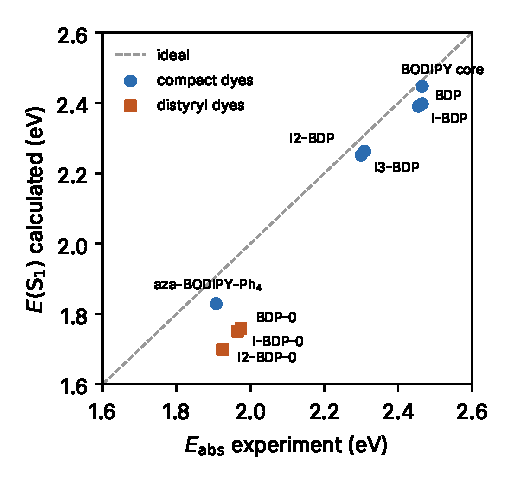
\includegraphics[width=0.48\textwidth]{figures/absorption_parity.pdf}
  \caption{Calculated S$_1$ (TDDFT+$\Delta$SCF) versus experimental absorption energy for the six
  compact dyes (circles) and the three distyryl dyes (squares).}
  \label{fig:abs}
\end{figure}

\section{Multireference results on the canonical (12e,11o) window}
The active orbitals are the canonical orbitals around the Fermi level (6 occupied, 5 virtual); see
Table~3 of the main text for their composition. CASCI and SC-NEVPT2 on RHF orbitals (Table~\ref{tab:cas},
Figure~\ref{fig:cas}); SA-CASSCF over three singlets with CASCI triplets on the same orbitals
(Table~\ref{tab:sanevpt2}); nested window growth, warm-started from the previous size
(Table~\ref{tab:sweep}). Scripts: \texttt{paper/references/run\_sa\_nevpt2.py} and \texttt{run\_cas\_sweep.py}.

\begin{table}
  \caption{S$_1$ excitation energies (eV) in the canonical (12e,11o) window on RHF orbitals, def2-SVP,
  compared with experiment and with the classical pipeline.}
  \label{tab:cas}
  \begin{tabular}{lcccc}
    \toprule
    Dye & exp & CASCI & SC-NEVPT2 & TDDFT+$\Delta$SCF \\
    \midrule
    BODIPY core    & 2.46 & 3.97 & 2.71 & 2.45 \\
    BDP            & 2.46 & 4.14 & 2.52 & 2.40 \\
    I2-BDP         & 2.31 & 4.32 & 2.04 & 2.26 \\
    aza-BDP-Ph$_4$ & 1.91 & 3.35 & 1.99 & 1.83 \\
    \bottomrule
  \end{tabular}
\end{table}
\begin{figure}
  \centering
  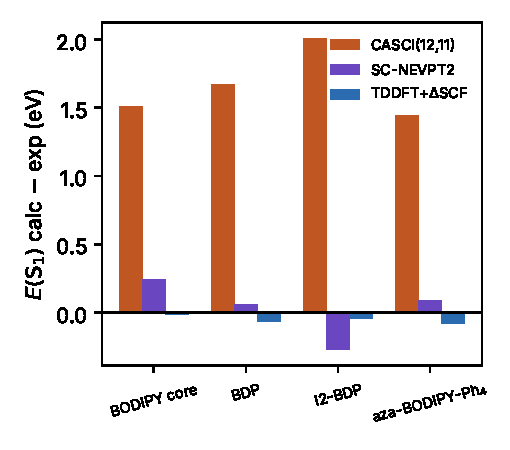
\includegraphics[width=0.48\textwidth]{figures/active_space_error.pdf}
  \caption{Error in the S$_1$ energy for CASCI(12e,11o), SC-NEVPT2 on the same active space, and the
  classical TDDFT+$\Delta$SCF pipeline.}
  \label{fig:cas}
\end{figure}
\begin{table}
  \caption{SA-CASSCF(12e,11o)/SC-NEVPT2 vertical energies (eV) on the canonical window, def2-SVP, gas
  phase, with experiment and the classical pipeline (T$_2-$S$_1$ from TDDFT T$_2$ and $\Delta$SCF S$_1$).}
  \label{tab:sanevpt2}
  \begin{tabular}{lcccccc}
    \toprule
    Dye & S$_1$ & S$_1$ exp & S$_1-$T$_1$ & S$_1-$T$_1$ exp & T$_2-$S$_1$ & T$_2-$S$_1$ TDDFT \\
    \midrule
    BODIPY core & 3.12 & 2.46 & 1.16 & --   & $+0.91$ & $+0.44$ \\
    BDP         & 3.05 & 2.46 & 0.99 & 0.77 & $+0.42$ & $+0.48$ \\
    I-BDP       & 2.99 & 2.46 & 1.03 & 0.76 & $+0.42$ & $+0.48$ \\
    I2-BDP      & 2.82 & 2.31 & 0.85 & 0.59 & $+0.37$ & $+0.32$ \\
    I3-BDP      & 2.83 & 2.30 & 0.80 & 0.58 & $+0.45$ & $+0.31$ \\
    aza-BDP-Ph$_4$ & 2.70 & 1.91 & 1.31 & --  & $+0.17$ & $+0.29$ \\
    \midrule
    BDP-0       & 2.49 & 1.97 & 1.00 & -- & $+0.50$ & $+0.53$ \\
    I-BDP-0     & 2.34 & 1.96 & 0.88 & -- & $+0.73$ & $+0.53$ \\
    I2-BDP-0    & 2.39 & 1.93 & 0.91 & -- & $+0.54$ & $+0.51$ \\
    \bottomrule
  \end{tabular}
\end{table}
\begin{table}
  \caption{Enlarging the canonical window for BDP and I2-BDP: vertical energies and gaps (eV),
  SA-CASSCF($n$,$n$) orbitals, def2-SVP. Experiment: S$_1$ 2.46 and 2.31~eV, S$_1-$T$_1$ 0.77 and 0.59~eV.}
  \label{tab:sweep}
  \footnotesize\setlength{\tabcolsep}{4pt}
  \begin{tabular}{llrrrrrr}
    \toprule
    & & \multicolumn{3}{c}{CASCI} & \multicolumn{3}{c}{SC-NEVPT2} \\
    Dye & ($n$,$n$) & S$_1$ & S$_1-$T$_1$ & T$_2-$S$_1$ & S$_1$ & S$_1-$T$_1$ & T$_2-$S$_1$ \\
    \midrule
    BDP    & (8,8)   & 3.80 & 1.74 & $-0.22$ & 3.08 & 1.00 & $+0.43$ \\
    BDP    & (10,10) & 3.22 & 1.17 & $+0.19$ & 3.02 & 0.99 & $+0.45$ \\
    BDP    & (12,12) & 3.06 & 1.03 & $+0.29$ & 2.97 & 0.96 & $+0.48$ \\
    BDP    & (14,14) & 3.06 & 1.03 & $+0.29$ & -- & -- & -- \\
    I2-BDP & (8,8)   & 3.16 & 1.08 & $+0.16$ & 2.84 & 0.82 & $+0.40$ \\
    I2-BDP & (10,10) & 2.94 & 0.94 & $+0.74$ & 2.86 & 0.87 & $+0.64$ \\
    I2-BDP & (12,12) & 2.94 & 1.07 & $+0.05$ & 2.84 & 0.88 & $+0.52$ \\
    I2-BDP & (14,14) & 2.94 & 1.07 & $+0.05$ & -- & -- & -- \\
    \bottomrule
  \end{tabular}
\end{table}

\section{Amplitude estimation on the filter circuit}
\begin{figure}
  \centering
  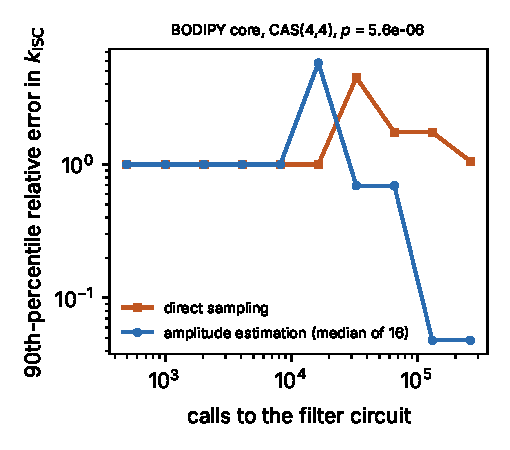
\includegraphics[width=0.48\textwidth]{figures/ae_demo.pdf}
  \caption{95th-percentile relative error of $\kisc$ against the number of calls to the filter circuit
  (BODIPY core, CAS(4,4), $p=5.6\times10^{-6}$): direct sampling, canonical amplitude estimation (median of
  16, ensemble over nearby amplitudes; crosses: circuit-level simulation at this $p$) and MLAE.}
  \label{fig:ae}
\end{figure}

\end{document}
